\chapter{Legge di Ampère-Maxwell}

Nei capitoli precedenti abbiamo trovato un'importante relazione tra il campo magnetico $\mathbf{B}$ e la corrente concatenata:

\begin{align}
    \oint_{C} \mathbf{B} \cdot d \mathbf{s} = \mu_0 i \\
    \nabla \times \mathbf{B} = \mu_0 \mathbf{j}
\end{align}

Questa relazione (riportata sia in forma integrale che differenziale) prende il nome di Legge di Ampère. \\

Quando abbiamo ricavato questa legge, però, abbiamo supposto di essere nel caso stazionario in cui $\nabla \cdot \mathbf{j} = 0$. Tuttavia nel caso generale vale l'equazione di continuità 

\begin{equation*}
    \nabla \cdot \mathbf{j} = - \frac{\partial \rho}{\partial t}
\end{equation*}

La quale, però, è in disaccordo con la legge di Ampère, infatti

\begin{equation}
    \nabla \cdot \mathbf{j} = \nabla \cdot \nabla \times \mathbf{B} = 0 \neq - \frac{\partial \rho}{\partial t}
\end{equation}

Ci è voluto il genio di J. C. Maxwell, stimolato dalle osservazioni di Faraday, per identificare la contraddizione e per modificare la legge di Ampère in una nuova legge che implica nuovi fenomeni, allora sconosciuti, ma in seguito osservati e verificati in dettaglio con gli esperimenti.\\

Ciò che Maxwell ha notato è il fatto che l'equazione di continuità si può convertire in una divergenza nulla usando la legge di Gauss, ossia 

\begin{equation}
    \nabla \cdot \mathbf{j} + \frac{\partial \rho}{\partial t} = \nabla \cdot \left( \mathbf{j} + \varepsilon_0 \frac{\partial \mathbf{E}}{\partial t} \right) = 0
\end{equation}

Maxwell ha quindi sostituito $\mathbf{j}$ nella legge di Ampère con la sua generaliazione 

\begin{tcolorbox}[colback=yellow!10!white, colframe=orange!70!black, boxrule=0.8pt]
\begin{equation}
    \mathbf{j} \to \mathbf{j} + \varepsilon_0\frac{\partial \mathbf{E}}{\partial t}
\end{equation}
\end{tcolorbox}

per campi dipendenti dal tempo. Pertanto le legge di Ampère si trasforma nella \emph{legge di Ampère-Maxwell} che diventa dunque 

\begin{tcolorbox}[colback=yellow!10!white, colframe=orange!70!black, boxrule=0.8pt]
\begin{equation}
    \nabla \times \mathbf{B} = \mu_0 \left( \mathbf{j} + \varepsilon_0 \frac{\partial \mathbf{E}}{\partial t} \right)
\end{equation}
\end{tcolorbox}

\newpage

mentre in foma integrale 

\begin{tcolorbox}[colback=yellow!10!white, colframe=orange!70!black, boxrule=0.8pt]
\begin{equation}
    \oint_{C} \mathbf{B} \cdot d \mathbf{s} = \mu_0 \int \left( \mathbf{j} + \varepsilon_0 \frac{\partial \mathbf{E}}{\partial t} \right) \cdot \mathbf{u}_n \ d\Sigma = \mu_0 (i + i_s) 
\end{equation}
\end{tcolorbox}

Dove $i_s$ è la corrente che si ottiene facendo l'integrale di superficie del primo termine e prende il nome di \emph{corente di spostamento}. \mkeyword{corrente di spostamento}

\section{Simmetria con la legge di Faraday}

Andiamo a considerare una regione di spazio in cui non ci sono correnti di conduzione ($i = 0$), ma ci sono variazioni di campo elettrico nel tempo, allora esiste un campo magnetico $\mathbf{B}$, determinato da 

\begin{tcolorbox}[colback=yellow!10!white, colframe=orange!70!black, boxrule=0.8pt]
\begin{equation}
    \oint_{C} \mathbf{B} \cdot d \mathbf{s} = \int_{\Sigma} \varepsilon_0 \mu_0 \frac{\partial \mathbf{E}}{\partial t} \cdot \mathbf{u}_n \ d\Sigma = \frac{1}{c^2} \frac{d \Phi (\mathbf{E})}{dt}
\end{equation}
\end{tcolorbox}

Dove abbiamo ulizzato l'espressione 

\begin{tcolorbox}[colback=yellow!10!white, colframe=orange!70!black, boxrule=0.8pt]
\begin{equation}
    c^2 = \frac{1}{\varepsilon_0 \mu_0}
\end{equation}
\end{tcolorbox}

Questo aspetto della legge di Ampère-Maxwell stabilisce una simmetria di comportamento con la legge di Faraday che prevede l'esistenza di un campo elettrico ove esistono variazioni di campo magnetico. 

\begin{figure}[h]
    \centering
    \begin{subfigure}{0.48\textwidth}
        \centering
        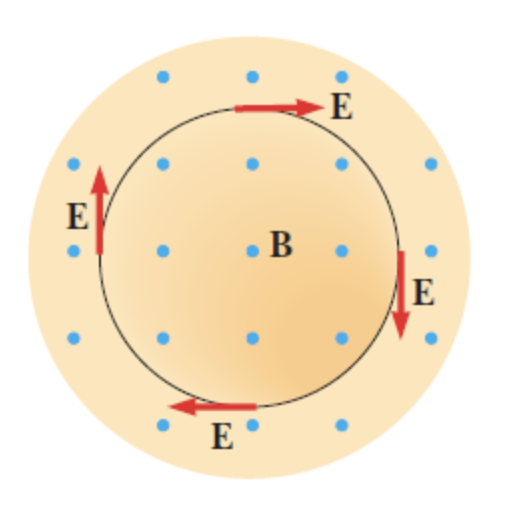
\includegraphics[width=0.7\linewidth]{figure/image64.png}
        \caption{$\oint_{C} \mathbf{E} \cdot d \mathbf{s} = - \frac{d \Phi(\mathbf{B})}{dt}$}
        \label{fig:sub1}
    \end{subfigure}
    \hfill
    \begin{subfigure}{0.48\textwidth}
        \centering
        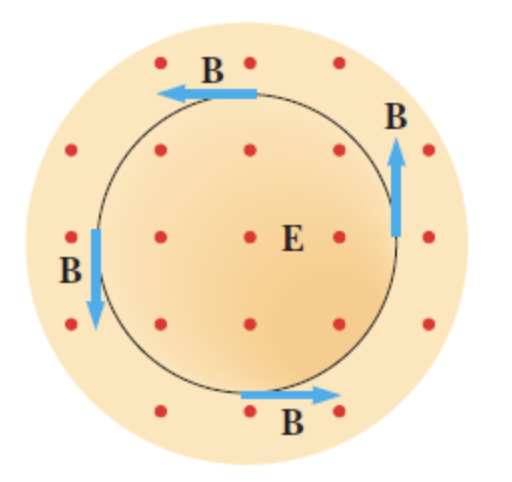
\includegraphics[width=0.7\linewidth]{figure/image65.png}
        \caption{$\oint_{C} \mathbf{B} \cdot d \mathbf{s} = \frac{1}{c^2} \frac{d \Phi(\mathbf{E})}{dt}$}
        \label{fig:sub2}
    \end{subfigure}
    %\caption{Confronto tra due campi elettrici}
    \label{fig:campi}
\end{figure}

\section{Campi magnetici quasi-statici ed effetto pelle} 